\begin{refsection}

\chapter{Constructing Spaces of Functions}
\label{chap:functionspaces}

\begin{tcolorbox}
This chapter provides an introduction to three popular machine learning techniques: kernel methods, Gaussian processes and neural networks. The material is expositional and is included for the reader's aid.
\end{tcolorbox}

A machine learning algorithm uses training data to select a function from a space of functions. In order for this procedure to work well, it is important to construct an appropriate space of functions for the algorithm to select from. When choosing a space of functions, there are three main considerations:
\begin{enumerate}
    \item \textit{Leveraging prior information.} How can prior knowledge or belief about the structure of the data be incorporated into the function space?
    
    \item \textit{Measuring complexity.} How can one assess the complexity of a function within the space, in order to choose a simple explanation of the data?
    
    \item \textit{Computational efficiency.} How can one design a space of functions that is cheap to select from in the face of data?
\end{enumerate}

This chapter surveys three popular techniques for constructing spaces of functions: kernel methods, Gaussian processes and neural networks. Each technique embodies a different philosophical approach to the above considerations. Kernel methods use \textit{functional analysis} to incorporate prior knowledge and measure complexity. Gaussian processes employ the tools of \textit{Bayesian probability}. While for neural networks, these considerations are mainly addressed via \textit{empiricism}---the proof of a method's validity is in its pudding.

While kernel methods, Gaussian processes and neural networks each take a different approach to the above questions, correspondences exist between their respective function spaces which allow tools from one to be ported to another. These correspondences are surveyed in Chapter \ref{chap:correspondences}. The present chapter focuses on introducing the function spaces themselves, their complexity measures and their approaches to fitting data.

Before moving on to the techniques, it will first be useful to define the notion of \textit{projecting} a function on to a set of inputs.

\begin{definition}[Function projection]\label{def:project} Given a function $f:\mathcal{X}\to\mathcal{Y}$ and a collection of $m$ inputs $X=\{x_1,...,x_m\}$, the \textit{projection} $f_X$ of the function $f$ on to the input data $X$ is given by:
\begin{equation}
    f_X \coloneqq \big[f(x_1), ..., f(x_m)\big] \in \mathcal{Y}^m.
\end{equation}
\end{definition}
In words: the projection of a function on to a set of inputs is the vector of function outputs across the inputs. Given a function $f(\cdot,w):\mathcal{X}\to\mathcal{Y}$ that is parameterised by a weight vector $w$, the projection on to $X$ is denoted $f_X(w)$.

\section{Kernel methods}

A kernel $k(\cdot,\cdot)$ is a function that measures the degree of similarity between its two arguments. In particular, when $k(x,x^\prime)$ is large then inputs $x$ and $x^\prime$ are similar, and when $k(x,x^\prime)$ is small then the two inputs are dissimilar. The notion of similarity is encoded by the choice of kernel function---a simple example being the Gaussian kernel:

\begin{example}[Gaussian kernel]\label{def:kgauss} For a pair of inputs $x,x^\prime\in\R^n$ and a length scale $\sigma>0$, the Gaussian kernel is given by:
\begin{equation}
    k_{\mathrm{Gaussian}}(x,x^\prime)\coloneqq \exp \left( - \frac{\|x-x^\prime\|_2^2}{2\sigma^2}\right).
\end{equation}
\end{example}

Beyond measuring similarity, a kernel may be used to construct a space of functions. To see this, consider that the Gaussian kernel viewed as a function of $x$ may be interpreted as an unnormalised Gaussian measure centred at the point $x^\prime$. The basic idea is that one may construct a more-or-less arbitrary function by superposing many Gaussian kernels centred at different locations. This idea is illustrated in Figure \ref{fig:kernel}. In accordance with this construction, the function $k_{\mathrm{Gaussian}}(\cdot,x^\prime)$ is referred to as the \textit{kernel basis function} centred at $x^\prime$.

\begin{figure}
    \centering
    \begin{minipage}[c]{0.38\textwidth}
    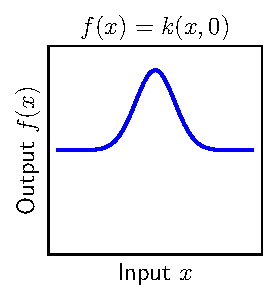
\includegraphics{figures/single_k.pdf}
    \end{minipage}
    \begin{minipage}[c]{0.22\textwidth}
    \begin{center}
        \Huge $\xrightarrow{\text{\normalsize superpose}}\;$
    \end{center}
    \end{minipage}
    \begin{minipage}[c]{0.38\textwidth}
    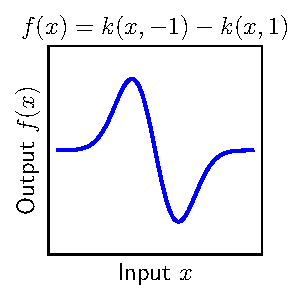
\includegraphics{figures/multi_k.pdf}
    \end{minipage}
    \caption[Constructing a function by superposing kernel basis functions]{Constructing a function by superposing kernel basis functions. The left panel displays a kernel basis function for the Gaussian kernel (Example \ref{def:kgauss}). The right panel shows how two kernel basis functions can be superposed to build a more complicated function. A \textit{reproducing kernel Hilbert space} (Definition \ref{def:rkhs}) consists of superpositions of arbitrarily many kernel basis functions.}
    \label{fig:kernel}
\end{figure}

By superposing kernel basis functions in this way, any kernel $k(\cdot,\cdot)$ can be used to construct a space of functions. The functions are parameterised by the centres and strengths of each kernel basis function within the superposition. Such a space of functions is known as a \textit{reproducing kernel Hilbert space} (RKHS). The remainder of this section will introduce the concept of an RKHS more formally, including how to measure the complexity of a function within an RKHS, and how to select a function from an RKHS in light of data.

\subsection{Using a kernel to construct a space of functions} 

For a function $k(\cdot,\cdot)$ to qualify as a kernel, it must satisfy two conditions:

\begin{definition}[Kernel]\label{def:kernel} A function $k:\mathcal{X}\times\mathcal{X}\to\R$ is a \textit{kernel} provided that:
\begin{enumerate}[label=\roman*)]
    \item $k$ is \textit{symmetric}: for any pair of inputs $x,x^\prime \in \mathcal{X}$, $k(x,x^\prime) = k(x^\prime, x)$;
    \item $k$ is \textit{positive definite}: for any set of $m$ distinct inputs $X=\{x_1,...,x_m\}$, the corresponding \textit{Gram matrix} $K_{XX}^{ij}\coloneqq k(x_i,x_j)$ is positive definite.
\end{enumerate}
\end{definition}
These conditions imply that important computations involving the kernel are well-defined. For instance, the inverse $K_{XX}^{-1}$ exists. Given Definition \ref{def:kernel}, it is simple to construct a space of functions by superposing kernel basis functions:

\begin{definition}[Pre-RKHS]\label{def:pre-rkhs} Given a kernel $k: \mathcal{X} \times \mathcal{X} \to \R$, the \textit{precursor} to a \textit{reproducing kernel Hilbert space} (pre-RKHS) consists of all linear combinations of finitely many kernel basis functions---that is, all functions of the form:
\begin{equation}
    f(\cdot)=\sum_{i=1}^m \alpha_i \, k(\cdot,x_i),
\end{equation}
for any weights $\alpha_1,...,\alpha_m\in\R$, centres $x_1, ..., x_m \in \mathcal{X}$, and positive integer $m$.
\end{definition}

One of the attractive features of a pre-RKHS is that one may measure the similarity of two functions within it by taking an inner product:

\begin{definition}[Pre-RKHS inner product] Given a kernel $k$ and two functions $f(\cdot) = \sum_{i=1}^m \alpha_i \,k(\cdot,x_i)$ and $g(\cdot) = \sum_{i=1}^{m^\prime} \beta_i\,k(\cdot,x_i^\prime)$, the \textit{inner product} of $f$ and $g$ in the pre-RKHS induced by $k$ is given by:
\begin{equation*}
    \langle f, g \rangle_\mathrm{RKHS} \coloneqq \sum_{i=1}^m \sum_{j=1}^{m^\prime} \alpha_i k(x_i,x_j^\prime) \beta_j \eqqcolon \alpha^\top K_{XX^\prime} \beta.
\end{equation*}
\end{definition}
It can be checked that, by the symmetry and positive definiteness of $k$, this definition serves as a valid inner product.

A standard treatment of kernel methods would now proceed to \textit{complete} the pre-RKHS to obtain a true \textit{Hilbert space} of functions. Completion essentially involves augmenting the pre-RKHS with certain limits of sequences of functions. This process adds significant technical overhead, while the pre-RKHS is already sufficient for the techniques studied in this thesis. As such, the term RKHS will be used herein merely as convenient shorthand for a pre-RKHS.

\begin{definition}[RKHS]\label{def:rkhs} By an abuse of terminology, an \textit{RKHS} is a pre-RKHS.
\end{definition}
\begin{definition}[RKHS inner product] By an abuse of terminology, an \textit{RKHS inner product} is a pre-RKHS inner product.
\end{definition}

Notice that the inner product of a function $f(\cdot) = \sum_{i=1}^m \alpha_i \,k(\cdot,x_i)$ with the kernel basis function $k(\cdot,x)$ \textit{reproduces} the function evaluated at $x$:
\begin{equation}\label{eq:reproducing}
    \langle f, k(\cdot,x) \rangle_{\mathrm{RKHS}} = \sum_{i=1}^m \alpha_i \,k(x,x_i) = f(x).
\end{equation}
Equation \ref{eq:reproducing} is known as the \textit{reproducing property} of the RKHS.

\subsection{Measuring complexity via RKHS norm}

The RKHS inner product also leads to a natural tool for measuring the complexity of functions within the RKHS: the RKHS norm.
\begin{definition}[RKHS norm]\label{def:rkhs-norm} Given a kernel $k$, the \textit{RKHS norm} of a function $f(\cdot) = \sum_{i=1}^m \alpha_i\,k(\cdot,x_i)$ in the RKHS induced by $k$ is given by:
\begin{equation*}
    \norm{f}_\mathrm{RKHS}^2 \coloneqq \langle f, f \rangle_\mathrm{RKHS} = \sum_{i=1}^m \sum_{j=1}^m \alpha_i k(x_i,x_j) \alpha_j \eqqcolon \alpha^\top K_{XX} \alpha.
\end{equation*}
\end{definition}

To demonstrate that the RKHS norm constrains the complexity of a function within an RKHS, the following lemma shows that the RKHS norm limits how fast a function can vary as its input is varied:

\begin{lemma} Consider a function $f:\mathcal{X}\to\R$ in an RKHS induced by kernel $k$. For any two inputs $x,x^\prime\in\mathcal{X}$, the variation in $f$ satisfies:
\begin{equation}
    \left|f(x) - f(x^\prime)\right| \leq \|f\|_\mathrm{RKHS} \cdot \mathrm{d}(x,x^\prime),
\end{equation}
where the distance function $\mathrm{d}(x,x^\prime)\coloneqq\sqrt{k(x,x) + k(x^\prime,x^\prime) - 2\cdot k(x,x^\prime)}$.
\end{lemma}
\begin{proof} By the reproducing property and the Cauchy-Schwarz inequality:
\begin{align*}
    \left|f(x) - f(x^\prime)\right| &= \left|\langle f, k(\cdot,x)-k(\cdot,x^\prime) \rangle_{\mathrm{RKHS}}\right|\\
    &\leq \|f\|_\mathrm{RKHS} \cdot \|k(\cdot,x)-k(\cdot,x^\prime)\|_\mathrm{RKHS}.
\end{align*}
The proof is completed by observing that, by the definition of RKHS norm, it holds that $\|k(\cdot,x)-k(\cdot,x^\prime)\|_\mathrm{RKHS}=\sqrt{k(x,x) + k(x^\prime,x^\prime) - 2\cdot k(x,x^\prime)}.$
\end{proof}
So a function's RKHS norm serves as a kind of \textit{Lipschitz constant} for the function's continuity. The distance between inputs in this notion of continuity is measured according to a special distance function $\mathrm{d}(\cdot,\cdot)$ related to the degree of kernel similarity between inputs. To gain further intuition about this lemma, it may help to consider its specialisation to the Gaussian kernel:
\begin{corollary}Consider a function $f:\mathcal{X}\to\R$ in the RKHS induced by the Gaussian kernel (Definition \ref{def:kgauss}) with length scale $\sigma=1$. For any two inputs $x,x^\prime\in\mathcal{X}$, the variation in $f$ satisfies:
\begin{equation}
    \left|f(x) - f(x^\prime)\right| \leq \sqrt{2} \cdot \|f\|_\mathrm{RKHS} \cdot \sqrt{1 - \econst^{-\half\|x-x^\prime\|_2^2}}.
\end{equation}
\end{corollary}

\subsection{Fitting data subject to minimum RKHS norm}

So far, this section has defined a space of functions called an RKHS, and a way to measure the complexity of functions in that space called the RKHS norm. It now makes sense to think of finding the least complex function in the RKHS that fits a set of data. This object admits a simple description, as follows:

\begin{theorem}[Minimum RKHS norm kernel interpolation]\label{thm:min-rkhs} Consider a set of $m$ distinct training inputs $X=\{x_1,...,x_m\}$ with respective training labels arranged into a vector $Y=[y_1,...,y_m]\in\R^m$. Say that a function $f$ \textit{interpolates} $(X,Y)$ if the projection $f_X$ (Definition \ref{def:project}) satisfies $f_X = Y$. In the RKHS induced by kernel $k$, the interpolator $f_\star$ of $(X,Y)$ with minimum RKHS norm is given by:
\begin{equation}\label{eq:min-rkhs-interpolator}
    f_\star(x) = \sum_{i=1}^m (K_{XX}^{-1} Y)_i\,k(x,x_i) \eqqcolon K_{xX} K_{XX}^{-1} Y,
\end{equation}
for Gram vector $K_{xX}^{i}\coloneqq k(x,x_i)$ and Gram matrix $K_{XX}^{ij}\coloneqq k(x_i,x_j)$.
\end{theorem}
\begin{proof}To see that $f_\star$ interpolates $(X,Y)$, observe that
\begin{equation*}
    [f_\star(x_1), ..., f_\star(x_m)] = K_{XX} K_{XX}^{-1} Y = Y.
\end{equation*}
To see that no interpolator exists with smaller RKHS norm, consider that another interpolator $g(\cdot)$ may be decomposed as:
\begin{equation*}
    g(\cdot) = f_\star(\cdot) + (g-f_\star)(\cdot).
\end{equation*}
But since $f_\star$ and $g$ both interpolate the training set, for any training input $x_i$:
\begin{equation*}
    \langle g-f_\star, k(\cdot,x_i) \rangle_\mathrm{RKHS}= g(x_i) - f_\star(x_i) =0,
\end{equation*}
where the first equality follows by the reproducing property. So $g-f_\star$ is orthogonal to kernel basis functions $k(\cdot,x_1),...,k(\cdot,x_m)$. Since $f_\star$ is constructed purely from those basis functions, this implies that $g-f_\star$ and $f_\star$ are themselves orthogonal: $\langle g-f_\star,f_\star\rangle_\mathrm{RKHS} = 0$. In turn:
\begin{equation}\label{eq:orthog-functions}
    \|g\|_\mathrm{RKHS}^2 = \|f_\star\|_\mathrm{RKHS}^2 + \|g-f_\star\|_\mathrm{RKHS}^2 \geq \|f_\star\|_\mathrm{RKHS}^2,
\end{equation}
which establishes the result.
\end{proof}

The implication of this theorem is that given a training set $S=(X,Y)$ of $m$ examples, the minimum RKHS norm interpolator $f_\star$ may be constructed by simple linear algebra operations $f_\star(x)=K_{xX} K_{XX}^{-1} Y$ involving kernel Gram matrix $K_{XX}$ and Gram vector $K_{xX}$. The dominant computational cost is that of inverting an $m \times m$ matrix, which is naïvely $\mathcal{O}(m^3)$. For this reason, the cost of kernel methods is typically cubic in the size of the training set.

Furthermore, Equation \ref{eq:min-rkhs-interpolator} shows that the kernel interpolator of minimum RKHS norm may be represented using only finitely many kernel basis functions. As such, Theorem \ref{thm:min-rkhs} is connected to a classic result known as the \textit{representer theorem} \citep{lwk}. 

\section{Gaussian processes}

The previous section showed that a function space may be constructed by superposing kernel basis functions. But there are other means of constructing a function space from a kernel. In the case of \textit{Gaussian processes}, a kernel is used to place a probability measure over a space of functions. The functions themselves may be sampled from this measure.

A probability measure on function space can be thought of as encoding \textit{prior belief} about which kinds of functions would have a good chance of explaining the data when it arrives. Phrased another way, functions of smaller prior probability might be considered more complex. An advantage of this approach is that, given the training data, a posterior distribution over functions consistent with the data may be constructed simply by turning the handle of Bayes' rule. This posterior provides not just a single prediction for a new data point, but a range of predictions each accompanied by a posterior probability.

\subsection{Constructing a space of functions by random sampling}

Given an input space $\mathcal{X}$, consider drawing a Gaussian random variable at each point $x\in\mathcal{X}$ and recording the value of each random draw as $f(x)\in\R$. To make life most interesting, one may choose not to draw these random variables independently, but rather from a joint Gaussian distribution. The covariance of this joint Gaussian could encode, for instance, that the closer an input $x$ is to another input $x^\prime$, the more likely it is that $f(x)$ would be similar to $f(x^\prime)$. This construction, of jointly Gaussian \textit{function values} $f(\cdot)$ with covariance structure based on similarity in the input space $\mathcal{X}$, is known as a Gaussian process:
\begin{definition}[Gaussian process]\label{def:gp} Consider an input space $\mathcal{X}$ and a kernel $k:\mathcal{X}\times\mathcal{X}\to\R$. If for any finite set of inputs $X=\{x_1, ..., x_m\}\in\mathcal{X}^m$, the distribution of function values $f(x_1),...,f(x_m) \sim \normal(0, K_{XX})$, then the function $f$ is drawn from a \textit{Gaussian process} with covariance $k$: $f\sim\gp(0,k)$.
\end{definition}
This definition is said to establish the \textit{prior measure} that a Gaussian process with a given kernel assigns to a space of functions.

\subsection{Measuring complexity via probability}
In principle, a Gaussian process provides a simple means to compare the complexity of functions. For instance, given two functions $f_1$ and $f_2$, one may simply declare the less likely of $f_1$ and $f_2$ under the Gaussian process prior to be more complex. To make this idea workable, one notices in Definition \ref{def:gp} that it is easier to assess the probability of a Gaussian process function when it is inspected only on a finite collection of inputs. As such, one could collect a collection of $m$ inputs $X\in\mathcal{X}^m$ and compare the density that $\normal(0,K_{XX})$ assigns to $\{f_1(x)\}_{x\in X}$ versus $\{f_2(x)\}_{x\in X}$. This procedure is not entirely satisfactory, since the answer depends on the choice of the set of inputs $X$. Still it conveys the spirit of the idea that prior probability may be used to assess complexity.

That being said, the complexity of individual functions does not usually play a major role in discussion of Gaussian processes. \textit{Distributions over functions} are considered to be more important, and Bayesians advocate for making predictions by integrating over these distributions of functions \citep{radford}. The next section will discuss how a posterior distribution may be constructed from the Gaussian process prior in light of data.

\subsection{Fitting data via Bayesian inference}

An attractive feature of Gaussian processes is that, given data, one may use Bayes' rule to derive a posterior distribution over functions. Given a training sample $S=(X,Y)$, Bayes' rule states that:
\begin{equation}\label{eq:bayes}
\Probe[f\mid S] = \frac{\Probe[S\mid f]\cdot \Probe[f]}{\sum_{f^\prime}\Probe[S\mid f^\prime]\cdot \Probe[f^\prime]}.
\end{equation}
There are three important quantities appearing in this equation:
\begin{enumerate}
    \item The \textit{prior} $\Probe[f]$ denotes the prior probability of function $f$.
    \item The \textit{likelihood} $\Probe[S\mid f]$ denotes how likely it is that a training sample $S=(X,Y)$ was obtained from a particular function $f$. The choice of likelihood is a modelling decision. The \textit{zero-one likelihood} is common:
    \begin{equation}\label{eq:zero-one-like}
        \Probe_{0/1}[S\mid f] \coloneqq \mathbb{I}[f(X) = Y].
    \end{equation}
    \item The \textit{posterior} $\Probe[f\mid S]$ denotes the probability of $f$ in light of the training sample under the choice of likelihood.
\end{enumerate}

\begin{figure}
    \centering
    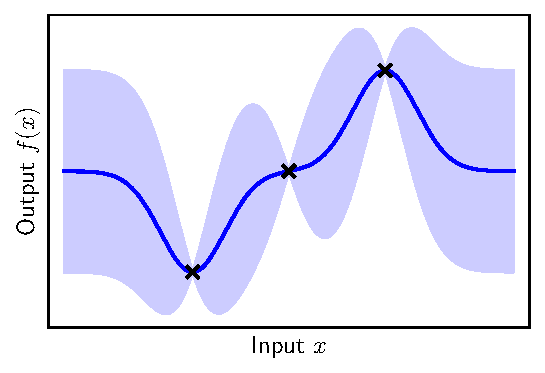
\includegraphics{figures/gp-var.pdf}
    \caption[Posterior distribution of a Gaussian process]{Posterior distribution of a Gaussian process, conditioned on fitting data marked by the black crosses. The kernel was set to the Gaussian kernel (Definition \ref{def:kgauss}) and the likelihood was set to zero-one (Equation \ref{eq:zero-one-like}). The solid blue line depicts the posterior mean, and the shaded region represents $\pm 1$ standard deviations about this mean.}
    \label{fig:gp}
\end{figure}

Bayesian inference is generally intractable due to the high-dimensional summation or integration that appears in the denominator of Equation \ref{eq:bayes}. But for Gaussian processes the required integrals are Gaussian in nature and often admit closed-form solutions. The following theorem is an important example:
\begin{theorem}\label{thm:gp-cond} Suppose that $f\sim\gp(0,k)$. Conditioned on $f$ interpolating dataset $(X,Y)$, the distribution of $f$ projected on to a fresh set of inputs $X^\prime$ is:
\begin{equation}\label{eq:gp-cond}
    f_{X^\prime} \sim \normal(K_{X^\prime X}K_{XX}^{-1}Y, K_{X^\prime X^\prime}-K_{X^\prime X}K_{XX}^{-1}K_{X X^\prime}).
\end{equation}
\end{theorem}
\begin{proof}
    Because $f\sim\gp(0,k)$, then $(f_X, f_{X^\prime})$ is jointly Gaussian with covariance $K_{X\cup X^\prime\,X\cup X^\prime}$ under this prior. The conditional distribution of this multivariate Gaussian, given that $f_X=Y$, is given by Equation \ref{eq:gp-cond} \citep{bishop}.
\end{proof}

Theorem \ref{thm:gp-cond} allows one to sample functions from the Gaussian process conditioned on interpolating a set of $m$ training examples. This process is illustrated in Figure \ref{fig:gp}. Just as was the case for kernel methods, the dominant computational cost is that of inverting the $m\times m$ kernel Gram matrix $K_{XX}$ which is naïvely $\mathcal{O}(m^3)$. This means that Gaussian processes, like kernel methods, are said to have a cost that is cubic in the size of the training set.

\section{Neural networks}

The function spaces corresponding to kernel methods and Gaussian processes are both derived starting from a kernel function. This renders certain global properties of their function spaces amenable to analysis---for instance, one can write down the kernel interpolator that \textit{globally minimises} the RKHS norm. Or one may write down a Gaussian process posterior distribution that includes within its support \textit{all functions} that interpolate a particular training set. Neural networks eschew these properties, in favour of something else.

A neural network function space is constructed by composing many operators, where each operator has a set of weights. Adjusting the weights in each operator adjusts the function realised by the entire network. The choice of operators and how they are connected to each other is referred to as the \textit{network architecture}. 

Given a particular neural network architecture, it has so far been hard to characterise global properties of the space of functions that it realises, unlike kernel methods and Gaussian processes. Though some things can be said in certain limiting regimes, as will be discussed in Chapter \ref{chap:correspondences}.

\begin{figure}
    \centering
    \def\layersep{2cm}
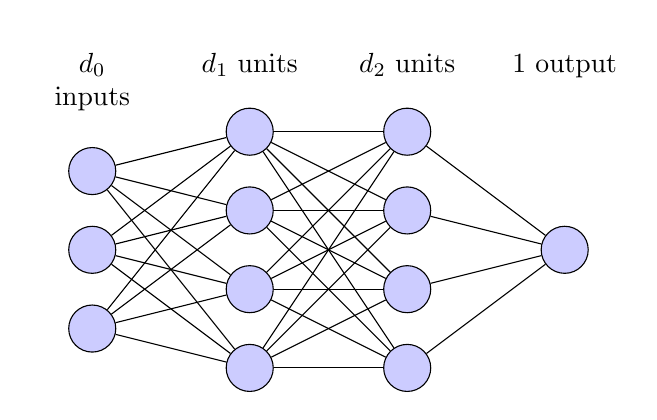
\begin{tikzpicture}[-,draw=black, node distance=\layersep]
    \tikzstyle{neuron}=[circle,draw=black,minimum size=17pt,inner sep=0pt,fill={rgb,255:red,204;green,204;blue,255}]
    \tikzstyle{annot} = [text width=4em, text centered, text height=3ex, text depth=3ex]

    \foreach \name / \y in {1,...,3}
        \node[neuron] (I-\name) at (0,-\y) {};

    \foreach \name / \y in {1,...,4}
        \path[yshift=0.5cm]
            node[neuron] (H-\name) at (\layersep,-\y cm) {};
            
    \foreach \name / \y in {1,...,4}
        \path[yshift=0.5cm]
            node[neuron] (H1-\name) at (\layersep*2,-\y cm) {};

    \node[neuron] (O) at (\layersep*3,-2 cm) {};

    \foreach \source in {1,...,3}
        \foreach \dest in {1,...,4}
            \path (I-\source) edge (H-\dest);
            
    \foreach \source in {1,...,4}
        \foreach \dest in {1,...,4}
            \path (H-\source) edge (H1-\dest);

    \foreach \source in {1,...,4}
        \path (H1-\source) edge (O);

    \node[annot,above of=H-1, node distance=0.75cm] (hl) {$d_1$ units};
    \node[annot,left of=hl] {$d_0$ inputs};
    \node[annot,right of=hl] (h2) {$d_2$ units};
    \node[annot,right of=h2] {$1$ output};
\end{tikzpicture}
    \caption[A multilayer perceptron]{A multilayer perceptron of depth $L=3$.}
    \label{fig:mlp}
\end{figure}

\subsection{Constructing a space of functions by composing parameterised operators}

The simplest example of a neural network architecture is the \textit{multilayer perceptron}---depicted in Figure \ref{fig:mlp}. The multilayer perceptron comprises a composition of matrices interspersed by elementwise nonlinearities, meaning that it encapsulates many of the key features of more general neural networks. As such, it will serve as a \textit{model organism} for detailed study in this thesis.

\begin{definition}[Multilayer perceptron]\label{def:mlp}
A \textit{multilayer perceptron} $f$ of depth $L$ maps an input $x\in\R^{d_0}$ to an output $f(x;w) \in \R^{d_L}$ via the map:
\begin{equation}\label{eq:mlp}
f(x; w) \coloneqq W_L \circ (\phi \circ W_{L - 1})\circ \dots \circ (\phi \circ W_1)\circ x.
\end{equation}
In this expression $\phi$ denotes an elementwise nonlinearity, $W_l$ denotes a matrix of dimension $d_l\times d_{l-1}$, and $w$ denotes the tuple of $L$ matrices $(W_1,...,W_L)$.
\end{definition}

Equation \ref{eq:mlp} provides a simple and direct means of constructing a space of functions. Without a nonlinearity, or with the nonlinearity set to the identity $\phi \gets \Id$, the overall function would be linear. The canonical choice of nonlinearity is known as the \textit{relu nonlinearity}:

\begin{definition}[Relu nonlinearity] The \textit{relu nonlinearity} is given by:
\begin{equation}
    \mathrm{relu}(\cdot) \coloneqq \max(0,\cdot).
\end{equation}
\end{definition}

So the relu nonlinearity retains the positive part of its input. It derives its name from the \textit{rectified linear unit}. The relu nonlinearity is both simple and works well in applications \citep{relu}.

\subsection{Measuring complexity via normalised margin}

Unlike kernel methods and Gaussian processes, the tools for studying the complexity of neural network functions are not yet mature. Developing such tools and their understanding is one of the aims of this thesis. That said, there have been some fairly natural proposals. In the case of a binary classification problem, the \textit{spectrally-normalised margin} is one such example:

\begin{definition}[Spectrally-normalised margin]\label{def:spec-norm-margin} Given a set of training data $S \in \{\R^{d_0}\times\pm 1\}^m$ and a multilayer perceptron $f:\R^{d_0}\times \mathcal{W}\to\R$ with matrices $w=(W_1,...,W_L)\in\mathcal{W}$, the \textit{spectrally-normalised margin} $\rho_\star$ is given by:
\begin{equation}\label{eq:spec-norm-magin}
    \rho_* \coloneqq \min_{(x,y)\in S} \frac{f(x;w)\cdot y}{\norm{x}_2\cdot\prod_{l=1}^L \norm{W_l}_*}.
\end{equation}
\end{definition}

The idea behind this definition is that, assuming that all training points are correctly classified, then the quantity $\min_{(x,y)\in S} f(x;w)\cdot y$ measures how close the closest training point is to being misclassified. But the problem with this measure is that a multilayer perceptron possesses various \textit{rescaling symmetries}---in particular, scaling up the input or a weight matrix at any layer scales up the margin too. Normalising by the product of norms that appear in the denominator of Equation \ref{eq:spec-norm-magin} yields a notion of margin that is invariant to these trivial rescaling symmetries. This definition of spectrally-normalised margin is related to one given by \citet{bartlett}.

Of course, there are other ways to measure margin modulo rescaling symmetries. For instance, the spectral norms appearing in Definition \ref{def:spec-norm-margin} measure the \textit{largest} singular value of each weight matrix in the multilayer perceptron. One may just as well measure the \textit{average} singular value. This motivates the following:

\begin{definition}[Frobenius-normalised margin]\label{def:frob-norm-margin} Given a set of training data $S \in \{\R^{d_0}\times\pm 1\}^m$ and a multilayer perceptron $f:\R^{d_0}\times \mathcal{W}\to\R$ with matrices $w=(W_1,...,W_L)\in\mathcal{W}$, let $\overline{d}_l\coloneqq \min(d_l,d_{l-1})$ be the minimum dimension of matrix $W_l\in\R^{d_l \times d_{l-1}}$. Then the \textit{Frobenius-normalised margin} $\rho_F$ is given by:
\begin{equation}
    \rho_F \coloneqq \min_{(x,y)\in S} \frac{f(x;w)\cdot y}{\norm{x}_2\cdot\prod_{l=1}^L \norm{W_l}_F/\sqrt{\overline{d}_l}}.
\end{equation}
\end{definition}
To understand this definition, note that the squared Frobenius norm $\norm{W_l}_F^2$ of a matrix is equal to the sum of its squared singular values. Also, a matrix $W_l$ has a number $\overline{d_l}$ of singular values in total. Therefore the Frobenius-normalised margin is just the spectrally-normalised margin with the largest singular value $\norm{W_l}_*$ replaced by the root-mean-square singular value $\norm{W_l}_F/\sqrt{\overline{d}_l}$. This definition is related to one given by \citet{my-margin}.

But what do these notions of normalised margin have to do with the complexity of a neural network function? Consider a neural network that perfectly classifies a particular training set $S$, but with very small normalised margin. This network is, in a sense, \textit{close} to a second network that misclassifies $S$. It would only take a small perturbation of the function realised by the former network to make it match the latter. Therefore, it seems reasonable that these two networks should have similar generalisation behaviour despite their differences on the training set. On the other hand, a network that classifies $S$ perfectly and with large normalised margin is not close to a network that misclassifies $S$. Based on this line of thinking, it may seem reasonable to declare networks with small normalised margin \textit{complex} on the grounds that they can mimic networks with different training error.

Of course, this is not a rigorous argument, and Definitions \ref{def:spec-norm-margin} and \ref{def:frob-norm-margin} are suggested only as candidate measures of complexity. Various modifications to these measures may work better. For example, one may consider replacing the minimum over the training set $\min_{(x,y)\in S}$ with the expectation $\Expect_{(x,y)\sim\uniform(S)}$. The role of these complexity measures in generalisation is studied further in Chapter \ref{chap:bpm}.

\subsection{Fitting data by gradient descent}

To use a neural network in a machine learning application, one needs a way of selecting a neural network that fits a particular training set. In the classification setting, a natural goal is to seek a neural network that perfectly classifies the training set. This could be measured by the \textit{zero-one loss}, say.

\begin{definition}[Zero-one loss]\label{def:zero-one-loss} For a neural network $f:\mathcal{X}\times\mathcal{W}\to\R$ and a training set $S\in(\mathcal{X}\times \pm 1)^m$, the \textit{zero-one loss} of weight vector $w\in\mathcal{W}$ is:
\begin{equation}
    \mathcal{L}_{0/1}(w) \coloneqq \frac{1}{m}\sum_{(x,y)\in S} \mathbb{I}[\sign f(x;w) \neq y].
\end{equation}
\end{definition}

Unfortunately, directly minimising the zero-one loss is not feasible, since its gradient with respect to the weights is either zero or undefined. Instead, a continuous proxy is used, such as the \textit{square loss}:

\begin{definition}[Square loss]\label{def:sq-loss} For a neural network $f:\mathcal{X}\times\mathcal{W}\to\R$ and a training set $S\in(\mathcal{X}\times \pm 1)^m$, the \textit{square loss} of weight vector $w\in\mathcal{W}$ is:
\begin{equation}
    \mathcal{L}_2(w) \coloneqq \frac{1}{2m}\sum_{(x,y)\in S} \left(f(x;w) - y\right)^2.
\end{equation}
\end{definition}

Observe that a neural network $f(\cdot,w)$ attaining square loss $\el_2(w) = 0$ also attains zero-one loss $\el_{0/1}(w)=0$. But the square loss can be conveniently minimised via gradient descent. In spirit, such a procedure is given by:
\begin{equation}
    w \gets w - \eta \cdot \nabla_w \el_2(w),
\end{equation}
where the constant $\eta>0$ denotes the user-prescribed learning rate. For computational efficiency, the gradient of the loss with respect to only a sub-sample of data is typically used, rather than with respect to the full dataset. This is referred to as either \textit{stochastic} or \textit{mini-batch} gradient descent. The theory of \textit{full-batch} gradient descent will be carefully studied in Part \ref{part:opt}. 

The square loss also admits a compact description via function projection:

\begin{proposition}[Square loss of projected function]\label{ex:sq-loss-projected} Consider a training set of $m$ examples $S=(X,Y)$. Let $f_X(w)$ denote the projection (Definition \ref{def:project}) of neural network $f(\cdot;w)$ on to $X$. The square loss may be written:
\begin{equation}\label{eq:sq-loss-projected}
    \el_2(w) = \frac{1}{2m}\cdot\norm{f_X(w)-Y}_2^2.
\end{equation}
\end{proposition}

Beyond square loss, other proxies for the zero-one loss are in use. For example:

\begin{definition}[Logistic loss]\label{def:log-loss} For a neural network $f:\mathcal{X}\times\mathcal{W}\to\R$ and a training set $S\in(\mathcal{X}\times \pm 1)^m$, the \textit{logistic loss} of weight vector $w\in\mathcal{W}$ is:
\begin{equation}
    \mathcal{L}_{\log}(w) \coloneqq \frac{1}{m}\sum_{(x,y)\in S} \log\left(1+\econst^{-y\cdot f(x;w)}\right).
\end{equation}
\end{definition}

The logistic loss is \textit{margin maximising} \citep{rosset2003margin}. This means that in contrast to the square loss, which is minimised by setting the training outputs to fixed values, the logistic loss is reduced by making the outputs on correctly classified training points larger in magnitude. 

A margin-maximising loss function would tend to increase the notions of normalised margin given in Definitions \ref{def:spec-norm-margin} and \ref{def:frob-norm-margin}---at least provided the norms of the weights in the network do not themselves grow. To prevent weight norms growing, an \textit{L2 penalty} is often added to the loss function:
\begin{definition}[L2 penalty]\label{def:l2-penalty} Given a neural network $f:\mathcal{X}\times\mathcal{W}\to\mathcal{Y}$ with $L$ layers and weight tuple $w=(W_1, ..., W_L)\in\mathcal{W}$, the \textit{L2 penalty} is given by:
\begin{equation}
    \norm{w}_2^2 \coloneqq \sum_{l=1}^L \norm{W_l}_F^2.
\end{equation}
\end{definition}
In words, the L2 penalty penalises the size of the Frobenius norm of the weight matrix at each layer. To train a network, one might then minimise the following \textit{L2-regularised} loss function:
\begin{equation}
    \el_{\mathrm{log}}(w) + \lambda \cdot \|w\|_2^2.
\end{equation}
This is often referred to as adding \textit{weight decay}, since in the gradient descent update the size of the weights are damped by a factor $(1-\eta \lambda)$ at each iteration:
\begin{equation}
    w \gets w \cdot (1 - \eta\lambda) - \eta \cdot \nabla_w \el_\mathrm{log}(w).
\end{equation}

The final comment of this chapter is that it has so far been difficult to theoretically characterise the computational cost of neural network training, although efforts have been made to obtain empirical scaling laws \citep{scaling-laws}. What can be said is that neural network training appears to overcome the unfavourable cubic cost of kernel methods and Gaussian processes.

\printbibliography[heading=subbibliography]
\end{refsection}